\section{Einleitung (Alle)}
Diese Arbeit beantwortet, ob NNs in der Softwaretechnik (SWT) eingesetzt werden können und wo die Grenzen der Anwendungen liegen. Die Arbeit ist keine Umfrage, ob NNs in der Realität eingesetzt werden. Vielmehr werden drei Themengebiete vorgestellt, in denen Forscher NNs testeten und einsetz\-ten. Das Ziel war es, anhand der Themengebiete und konkreter Beispiele herauszufinden, ob und wie NNs in der SWT eingesetzt werden können.
NNs basieren auf der Funktion des biologischen Nervensystems. Informationen werden, wie bei einem menschlichen Gehirn auch, durch eine Vielzahl miteinander verknüpfter parallel laufender Neuronen  verarbeitet. Die daraus entstehenden Systeme trainieren sich teilweise selbst, um schnellere Entscheidungen treffen und Fehler vermeiden zu können~\cite{technology}. 
In dieser Arbeit wird näher auf CNNs und Resnets eingegangen. CNNs werden im Kapitel Spracherkennung näher erläutert, da die aufgeführten Beispiele auf CNNs bevorzugt eingehen. Resnets gehören zur Kategorie der DNNs. Jeder Layer des Resnets stellt ein sogenanntes \textit{Res} dar und besitzt mehrere trainierbare Neuronen. Neuronen sind in Bezug auf NNs Leiter und Überträger von Daten und Werten. Das Besondere ist der Dropout, welcher durch zufälliges Ausschalten von Neuronen Überanpassungen derselbigen vermeidet ~\cite{residualnn}. Mehrschichtige neuronale Netze (Multilayer perceptrons) benutzen u.a. Back propagation, um Parameter für künstliche neuronale Netze zu trainieren. Back propagation dient dem Trainieren von Layern, genauer dessen Neuronen, um auf entstandene Fehler aufmerksam zu machen, welche rückwärts durch das NN gegeben werden, um die sogenannten shared weights neu auszurichten~\cite{usingcnn}.\\
\vspace{6.0cm}

\section*{Neuronale Netze}
NNs werden verwendet, um unübersichtliche und komplizierte Probleme zu lösen. NNs bestehen aus Knotenelementen, den sog. Neuronen. Mehrere Neuronen bilden einen Layer. Bei herkömmlichen NNs wird zwischen den drei Layerarten Input-, Hidden- und Outputlayer unterschieden. Input- und Outputlayer sind in einem NN genau ein Mal vorhanden und dienen der Ein- und Ausgabe des NN. Zwischen diesen Schichten befinden sich beliebig viele Hiddenlayer. Jedes Neuron besitzt eine Verbindung zu allen Neuronen der folgenden Schicht. Von der jeweils oberen Schicht werden über diese Verbindungen Signale an die darunterliegende Schicht weitergeleitet. Eine Aktivierungsfunktion entscheidet in jedem Neuron, ob die eingetroffenen Signale für eine Weiterleitung ausreichen. Auf den Verbindungen liegen unterschiedliche Gewichtungen, die die Intensität eines Signals be\-einflussen. Beim Training des NN werden die Gewichtungen angepasst.
Es gibt zwei grundsätzliche Trainingsansätze. Das supervised learning setzt einen Datensatz mit erwarteten Ergebnissen voraus. Nach Verarbeitung der Daten werden die Gewichte des NN anhand der Erwartungswerte angepasst. Ansätze für unsupervised learning kommen auch ohne gekennzeichnete Daten aus, sind aber derzeit noch nicht einsatzfähig. NNs können durch ihre Fähigkeit dazuzulernen komplexe Sachverhalte verarbeiten und bieten einen Lösungsansatz für zuvor unlösbare Probleme~\cite{Maind2014}.\\
\begin{figure}[h]
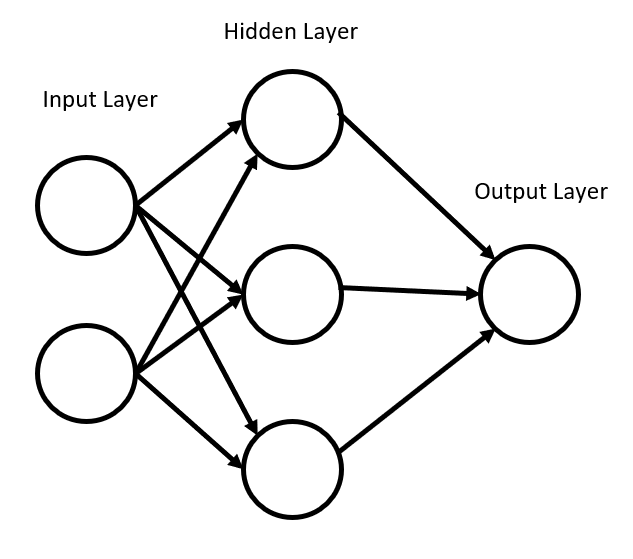
\includegraphics[width=\linewidth, height=6cm]{Bilder/NN/NeuralNetwork.png}
\caption{NN-Architektur vgl.~\cite{Maind2014}}
\end{figure}
\\
\\
\\
\\
In Kapitel \ref{Mustererkennung} wird die Disziplin Mustererkennung und dazugehörige Verfahren und Möglichkeiten näher beschrieben. Anschließend wird in Kapitel \ref{KostenAufwand} der Einsatz von NNs im Gebiet Kosten- und Aufwandsschätzung erläutert und damit verbundene Methoden und Praktiken aufgezeigt. Kapitel \ref{SQ} befasst sich mit NNs im Bereich Qualitätsmanagement und gibt einen Einblick auf verwendete Mittel und Vorgehensweisen, welche in dem genannten Bereich notwendig und nützlich sind. Letztendlich folgt ein Fazit, welches die Ergebnisse aus allen Kapiteln vereint, vergleicht und bewertet.